\section{Major examples fitting this architecture.} \label{generality}

The notation of equation~(\ref{eq-recurrent}) seems to be the most general form of usual recurrent networks. Let us state this point by considering several examples of units, and make explicit how we decompose them in term of nodes.

\paragraph{Linear non-linear (LNL) units.} 

Such network unit corresponds to the most common\footnote{See also a dual form related to AIF, in the sequel, with an alternate insertion of the non-linearity.} network unit and is defined by a recurrent equation of the form:
\begin{equation}\label{lnl-network}
\begin{array}{rcl}x_n(t) &=& \gamma_n \, x_n(t-1) \\ &+& \zeta_{[a,b]}\left(\alpha_n + \sum_{n' = 0}^{N-1} W_{nn'} \, x_{n'}(t-1) + \sum_{m = 0}^{M-1} W_{nm} \, i_m(t-1)\right), \end{array}\end{equation}
\\- with either a fixed or adjustable {\em leak}\footnote{Here $\gamma = 1 - \frac{\Delta T}{\tau}$ stands for the leak of each unit, writing $\Delta T$ the sampling period, $\tau$ the continuous leak and using an basic trivial Euler discretization scheme, the $\zeta()$ profile being re-normalized accordingly.} $\gamma_n$, providing $0 < \gamma_n < 1$, and 
\\- optionally {\em intrinsic plasticity} parameterized by $\alpha_n$. 

The {\em non-linearity} often\footnote{If the model corresponds to a rate, i.e., a firing probability, we can use the logistic sigmoid, which writes $\zeta_{[0,1]}(u) = \frac{1}{1 + e^{-4 \, u}} = \frac{1 + \tanh(2 \, u)}{2}$.} writes
\eqline{\zeta_{[a,b]}(u) \deq \frac{a+b}{2} + \frac{b-a}{2} \, \tanh(\frac{2}{b-a} \, u),}
with $\zeta_{[a,b]}(-\infty) = a, \zeta_{[a,b]}(+\infty) = b, \zeta_{[a,b]}(u) = \frac{a+b}{2} + u + O(u^3)$,  while $\zeta'(u) = 1 - \tanh(\frac{2}{b-a} \, u)^2$,  $0 < \zeta'(u) \leq 1$, with $\max|\zeta'(u)| = 1$, thus contracting with a correct numerical conditioning. We mainly have $[a,b] = [0,1]$ or $[a,b] = [-1,1]$ depending on the semantic interpretation of the $x_n(t)$ variable.

Another form of non-linearity is a rectified linear unit (or ReLU), i.e.:
\eqline{\zeta_{[0,+\infty]}(u) \deq \max(0, u).}
This function is not derivable at $u = 0$. It is however very easy to consider a mollification (called ``softplus'') e.g., $\zeta_{\epsilon, [0,+\infty]}(u) \deq \epsilon \, \log\left(1 + e^{\frac{u}{\epsilon}}\right)$ which is an analytic smooth approximation which uniformly converges\footnote{Since $\forall u, |\zeta_{\epsilon, [0,+\infty]}(u) - \zeta_{[0,+\infty]}(u)| \leq \log(2) \, \epsilon$.}, i.e. $\lim_{\epsilon \rightarrow 0} \zeta_{\epsilon, [0,+\infty]}(u) = \zeta_{[0,+\infty]}(u)$. See the section on AIF units to see how to adjust, if needed, such a meta-parameter redefining it as a node parameter.

For adjustable leak we need three nodes to fit within the proposed notations:
\eqline{\begin{array}{rcl}
 x_n(t) &=& x_{n_1}(t) + \zeta_{[a,b]}\left(x_{n_2}(t)\right) \\
 x_{n_1}(t) &=& \gamma_n \, x_{n}(t-1) \\
 x_{n_2}(t) &=& \alpha_n + \sum_{n' = 0}^{N} W_{nn'} \, x_{n'}(t-1) + \sum_{m = 0}^{N} W_{nm} \, i_m(t-1) \\
\end{array}}
and it is easy to verify that this second form fits with equation~(\ref{eq-recurrent}), since:
\\- The 1st line corresponds to a parameter-less $\Phi_{n0t}\left(\right)$ kernel (unit firmware).
\\- The 2nd and 3rd lines correspond to linear combinations of elementary kernels $\Phi_{ndt}\left(\right)$ selecting another state or input variable (unit learnware).

With this example, we see that the proposed approach is to introduce two additional intermediate variables $x_{n_1}(t)$ and $x_{n_2}(t)$ related to each linear combination of weights or other parameter.

With a fixed leak (i.e., if the value $\gamma_n$ is known) the LNL unit decomposes into two nodes, a parameter less node combining $x_n(t)$ and $x_{n_1}(t)$, and the linear combination defined for $x_{n_2}(t)$.

This equation is also valid for the main auto-encoder architectures, and for convolution networks \cite{Bengio:2009,Deng:2014}, with an important additional feature : weight-sharing, i.e. the fact that several weights $W_{nd}$ are the same across different nodes. This is taken into account in this paper.

\paragraph{Long short term memory (LSTM) units.} 

Such network unit is defined by a sophisticated architecture \cite{Hochreiter:1997}, described in figure~\ref{recurrent-network}. A unit is made of the following nodes:
\begin{equation}\label{lstm-network}
\begin{array}{rcl}
\multicolumn{3}{l}{\mbox{Unit output:}} \\
x_n(t) &=& \zeta_{[0,1]}\left(y_n^{out}(t)\right) \, \zeta_{[-1,1]}\left(s_n(t)\right) \\
\multicolumn{3}{l}{\mbox{Unit state:}} \\
s_n(t) &=& \zeta_{[0,1]}\left(y_n^{forget}(t)\right) \, s_n(t-1) + 
          \zeta_{[0,1]}\left(y_n^{in}(t)\right) \, \zeta_{[-1,1]}\left(g_n(t)\right) \\
\multicolumn{3}{l}{\mbox{Unit gate:}} \\
g_n(t) &=& \sum_{n'} W^g_{nn'} \, x_{n'}(t-1) + \sum_{m} W^g_{nm} \, i_m(t-1) \\
\multicolumn{3}{l}{\mbox{Output modulation:}} \\
y_n^{out}(t) &=& W^o_n \, s_n(t-1) + \sum_{n'} W^o_{nn'} \, y_{n'}^c(t-1) + \sum_{m} W^o_{nm} \, i_m(t-1) \\
\multicolumn{3}{l}{\mbox{Forgetting modulation:}} \\
y_n^{forget}(t) &=& W^f_n \, s_n(t-1) + \sum_{n'} W^f_{nn'} \, y_{n'}^c(t-1) + \sum_{m} W^f_{nm} \, i_m(t-1) \\
\multicolumn{3}{l}{\mbox{Memorizing modulation:}} \\
y_n^{in}(t) &=& W^i_n \, s_n(t-1) + \sum_{n'} W^i_{nn'} \, y_{n'}^c(t-1) + \sum_{m} W^i_{nm} \, i_m(t-1)  \\
\end{array}\end{equation}

The first two nodes are parameter-less additive and/or multiplicative combination of non-linear functions of the reminding four nodes, which are themselves linear combination of the incoming signal gate and the input, forgetting and output modulatory signals. 

The present notation corresponds to the most general form (e.g., with peephole connections \cite{Gers:2003}) of LSTM, while several variants exist. A rather closed mechanism is named gate recurrent unit \cite{Cho-2014}, and is based on the same basic ideas of modulatory combination, but with a simpler architecture. We do not make explicit the equations for all variants of LSTM here, just notice that they correspond to some of the very best solutions for high performance recurrent network computation \cite{Schmidhuber:2015}.

\begin{figure}[!ht]
  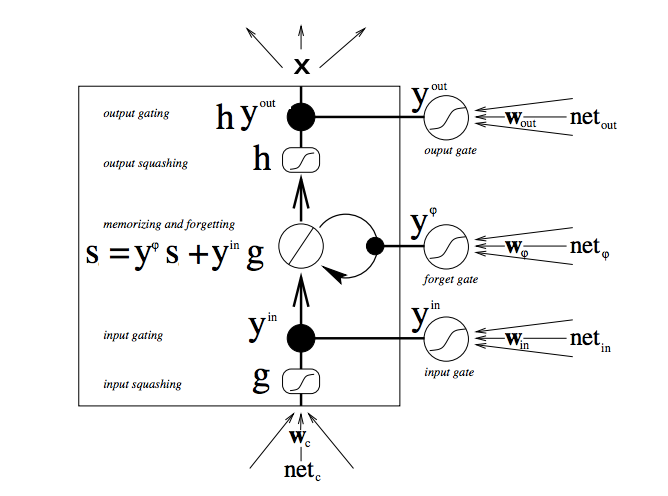
\includegraphics[width=0.8\textwidth]{img/lstm-unit}
  \caption{A LSTM unit has three processing stages for bottom to top: The (i) gate $g$ corresponds to as standard LNL unit that (ii) feeds an internal state memory $s$ which value is also driven by a forget (or remember) signal allowing to maintain the previous value, before (iii) the output connected value $x$ diffuse (or not) the result in the network. The LSTM mechanism is thus based on three ingredients, (a) the use of modulatory connection (i.e., with a multiplication by a number between 0 and 1 in order to control the signal gain), (b) a memory ``carrousel'' (i.e., an equation that could be of the form $s_n(t) = s_n(t-1)$ in order to maintain a signal, during a long short-term delay), and (c) the use of several modulatory signals. From \cite{Hochreiter:1997}.}
  \label{lstm-unit}
\end{figure}

However, in our context, instead of reusing such a complex unit as it, the design choice is to consider the non standard nodes (i.e., unit output and unit state) as modular nodes that could be combined with NLN at different level of complexity, depending on the task. At the implementation level we are not going to provide LSTM units as black boxes but an object-oriented framework allowing to adjust the network architecture to the dedicated task.

A key-point is that LSTM have, by construction, a real virtue regarding weight adjustment since back-propagation curses (vanishing or explosion) is avoided \cite{Schmidhuber:2015}. A strong claim of this paper is that we can efficiently adjust the recurrent network weights even if we do not use (or only use) LSTM but simpler units also.

\paragraph{Strongly-Typed Recurrent Neural units.} 

This other formalism \cite{Balduzzi:2016} carefully considers the signal type in the sense of parameters of different physical origins (e.g., Volts and meter), that cannot be simply mixed. This approach allows unary and binary functions on vectorial values of the same type, transformation from one orthogonal basis to another (thus using orthogonal matrices only) and component-wise product (i.e., modulatory combination). The authors show that strongly-typed gradients better behaved and that, despite being more constrained, strongly-typed architectures achieve lower training and comparable
generalization error to classical architectures. Considering a strongly-typed LNL unit, following \cite{Balduzzi:2016} and translating in the present notation, at the same degree of generality of LNL networks, we obtain:
\begin{equation}\label{st-lnl-network}\begin{array}{rcll}
  x_n(t) &=& \zeta_{[0,1]}\left(f_n(t)\right) \, x_n(t-1) + \left(1 - \zeta_{[0,1]}\left(f_n(t)\right)\right) \, z_n(t) \\
  f_n(t) &=& \alpha_n + \gamma_n \,  x_n(t-1) \\
  z_n(t) &=& \sum_{n' = 0}^{N} W'_{nn'} \, x_{n'}(t-1) + \sum_{m = 0}^{N} W'_{nm} \, i_m(t-1) \\
\end{array}\end{equation}
The first line is the firmware combination of the unit forgetting mechanism, this value being defined in the 2nd line, while the 3rd line performs the linear combination of other network values.
It is an interesting alternative to usual approach, embedable in our notation.

\paragraph{Approximation of {\em leaky integrate and fire} (AIF), current-driven, spiking-neuron unit.}

Let us also discuss how to cope with spiking networks (see \cite{cessac-paugam-moisy-etal:10} for a general discussion on such network computational power and limit).
 Following \cite{cessac_discrete_2008} (with a tiny change of notation), we consider without loss of generality a discretized form, which writes: \begin{equation}\label{lif-network} \begin{array}{rcl}x_n(t) &=& \gamma_n \, \left(1 - \Upsilon_\epsilon\left(x_n(t-1)\right)\right) \,x_n(t-1) \\ &+& \sum_{n' = 0}^{N} W_{nn'} \, \Upsilon_\epsilon\left(x_{n'}(t-1)\right) + \sum_{m = 0}^{N} W_{nm} \, i_m(t-1), \end{array}\end{equation} 
where the unit value is over or below the spiking threshold $\theta = 1/2$ (thus spiking or not), while the reset value is $0$.

Here, as inspired from \cite{cessac_using_2012}, we propose to use $\Upsilon_\epsilon(v) \deq \zeta_{[0,1]}\left(\frac{v-1/2}{\epsilon}\right)$, as a mollification of the threshold function\footnote{Obviously, $\lim_{\epsilon \rightarrow 0, v \neq 0} \Upsilon_\epsilon(v) = \Upsilon(v)$, while $\Upsilon'_\epsilon(0) = 1/\epsilon$ and $\int_v |\Upsilon_\epsilon(v) - \Upsilon(v)| = \log(2)/2 \, \epsilon$. Here the convergence can not be uniform (since a continuous function converges towards a step function), more precisely $\sup_v |\Upsilon_\epsilon(v) - \Upsilon(v)| = 1/2$ (around $v\simeq 1/2$). 
}: 
\eqline{\Upsilon(v) \deq \left\{\begin{array}{cl} 0 & v < 1/2 \\ 1/2 & v = 1/2 \\ 1 & 1/2 < v \\ \end{array}\right..}
To avoid spurious effects when adjusting the weights, we have to find out the best minimal $\epsilon$ value for each unit.

As far as the unit architecture is concerned, it is a simple variant of LNL unit, with different kernel function, and different positioning of the non-linearity. The key point is that this so called BMS formulation fits with the present approach:
\eqline{\begin{array}{rcl}
 x_n(t) &=& \gamma_n \, \left[(1-\zeta_{[0,1]}(x_{n_1}(t))) \, x_n(t-1)\right] \\ 
  &+& \alpha_n + \sum_{n' = 0}^{N} W_{nn'} \, \zeta_{[0,1]}\left(x_{n'_1}(t-1)\right) + 
      \sum_{m = 0}^{N} W_{nm} \, i_m(t-1) \\
 x_{n_1}(t) &=& \frac{1}{\epsilon} \, \left[x_n(t-1) - \frac{1}{2} \right] \\
\end{array}}
Here $\omega\deq\frac{1}{\epsilon}$ is now a parameter to estimate, in order each unit to be a suitable approximation of a spiking activity. This differs from \cite{cessac_using_2012} where sharpness was considered as a meta-parameter: Here it is a parameter learned on the data. In both cases, we need ${\epsilon \rightarrow 0}$, which means that the transformation is very sharp, limiting the numerical stability. This is going to be investigated at the numerical level.

The use of such units is very interesting in practice and we review in appendix~\ref{closedforms} how they can be used to propose trivial solutions to rather complex tasks.

\paragraph{Softmax and exponential probability units.} 

When considering exponential distribution of probability on one hand, or softmax\footnote{
The relation with a max operator comes from the fact that:
\eqline{x_n(t) \deq \frac{e^{\frac{z_n(t)}{\epsilon}}}{\sum_n e^{\frac{z_n(t)}{\epsilon}}} \Rightarrow \lim_{\epsilon \rightarrow 0} \sum_n x_n(t) \, z_n(t) = \max_n \left( z_n(t)\right).}
In words the softmax weighted sum of values approximates these values maximum.} computation on the other hand, one comes to the same equation\footnote{See, e.g., \url{https://en.wikipedia.org/wiki/Softmax\_function}.} which writes: \begin{equation}\label{exp-network}\begin{array}{rcl}
x_n(t) &=& \frac{e^{z_n(t)}}{\sum_n e^{z_n(t)}} = \exp\left(z_n(t) - \log(\sum_n \exp\left(z_n(t)\right)\right) \\
z_n(t) &=& \alpha_n + \sum_{n' = 0}^{N} W'_{nn'} \, x_{n'}(t-1) + \sum_{m = 0}^{N} W_{nm} \, i_m(t-1) \\
\end{array} \end{equation} with $\sum_n x_n(t) = 1$ in relation with the so-called partition function $Z(t) = \sum_n \exp\left(z_n(t)\right) > 0$. 

This kind of unit, in addition to NLN units, or LSTM units form the basic components of deep-learning architectures \cite{Bengio:2009,Deng:2014}.

The 1st line is a firmware global equation\footnote{It is worthwhile mentioning that:
\eqline{\partial_{z_{n'}(t)} o_n(t) = o_n(t) \, \left(\delta_{n=n'} - o_{n'}(t)\right) \in [0,1], \delta_{n=n'} = \left\{\begin{array}{cl} 1 & n = n' \\ 0 & \mbox{otherwise} \end{array}\right.,}
thus numerically well defined, with no singularity, the transformation being contracting, i.e., $\left|\partial_{{\bf z}} {\bf o}\right| \leq 1$, with $\max|\partial_{{\bf z}} {\bf o}|=1$.} which is a function of all units value of the same layer.

We encounter such a construction in restricted Boltzmann machine (RBM) (also using LNL network with the logistic sigmoid, but in a context of stochastic activation of the units in this case) \cite{Bengio:2009}. We mention this possibility for the completeness of the discussion, making explicit the fact that the present framework includes such equation. However, the estimation problem addressed in RBM completely differs (as being a stochastic estimation paradigm) from the deterministic estimation considered here, the key difference being the fact we want relevant results event on small data sets.

\paragraph{Other aspects of the proposed notation} 

It is also straightforward to verify that the reservoir computing equations \cite{verstraeten-etal:07} also fit with this framework, as being a particular of LNL network, since they simply correspond to a recurrent reservoir of interconnected units, plus a read-out layer.

Since there is no restriction on the architecture, depending on the choice of the kernels, it also can represent a two-layers non-linear network, or even better a multi-layers deep network. The trick is simply to choose kernels corresponding to the desired inter-layer and intra-layer connectivity.

A step further, in a given architecture, we can adjust both the number of layers and the choice between one or another computation layer. This aspect if further discussed in \cite{Drumond2017From}. We also would like to consider not only a sequence of layers, but a more general acyclic graph of layers, noticing that shortcuts can strongly improve the performance thanks to what is called residual-learning \cite{He2016Deep}. Following \cite{Fdrumond2017}, the key-point is that we want to have this structural optimization as a parameter continuous adjustment and not a meta-parameter combinatory adjustment. The proposal is thus to consider an architecture with {\em versatile layers} where the choice of the non-linearity is performed via a linear combination, obtained with sparse estimation, thus acting as a soft switch. Furthermore, adding shortcuts allows to define an adjustable acyclic graph with the output as supremum and the input as infimum. On the reverse, \cite{Fdrumond2017} points out that any acyclic graph can obviously be defined in this framework. Of course, we do not expect this method to generate the best acyclic graph and combination of modules, but to improve an existing architecture by extending usual optimization to the exploration of structural alternatives.

